% figures/domain_layers.tex -- Layer distribution across cognitive domains
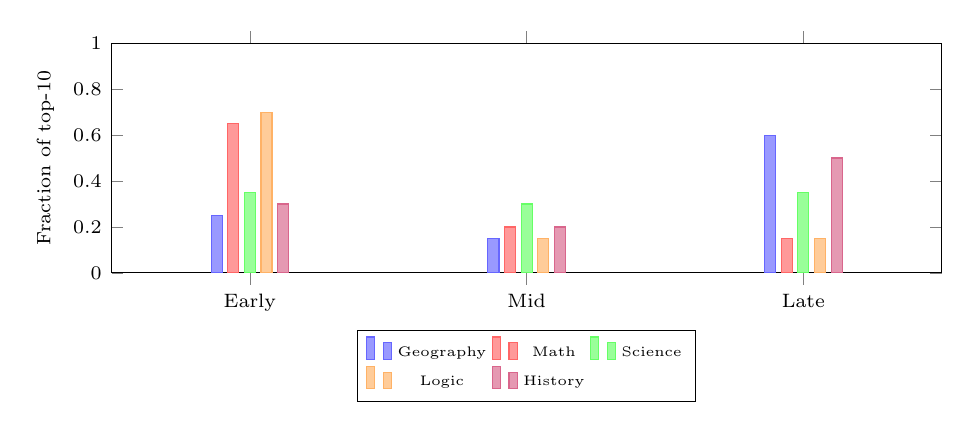
\begin{tikzpicture}
\begin{axis}[
    ybar,
    width=\columnwidth,
    height=4.5cm,
    bar width=4pt,
    ylabel={Fraction of top-10},
    symbolic x coords={Early, Mid, Late},
    xtick=data,
    x tick label style={font=\scriptsize},
    y tick label style={font=\scriptsize},
    ylabel style={font=\scriptsize},
    legend style={
        font=\tiny,
        at={(0.5,-0.25)},
        anchor=north,
        legend columns=3
    },
    ymin=0, ymax=1,
    enlarge x limits=0.25,
    nodes near coords={}
]

\addplot[fill=blue!40, draw=blue!60] coordinates {
    (Early, 0.25) (Mid, 0.15) (Late, 0.60)
};
\addplot[fill=red!40, draw=red!60] coordinates {
    (Early, 0.65) (Mid, 0.20) (Late, 0.15)
};
\addplot[fill=green!40, draw=green!60] coordinates {
    (Early, 0.35) (Mid, 0.30) (Late, 0.35)
};
\addplot[fill=orange!40, draw=orange!60] coordinates {
    (Early, 0.70) (Mid, 0.15) (Late, 0.15)
};
\addplot[fill=purple!40, draw=purple!60] coordinates {
    (Early, 0.30) (Mid, 0.20) (Late, 0.50)
};

\legend{Geography, Math, Science, Logic, History}

\end{axis}
\end{tikzpicture}
